\documentclass[11pt,letterpaper]{article}

\usepackage[margin=1in]{geometry}
\usepackage{amsmath,amssymb}
\usepackage{graphicx}
\usepackage{subcaption}
\usepackage{booktabs}
\usepackage{hyperref}
\usepackage{enumitem}
\usepackage{microtype}
\usepackage{xcolor}
\usepackage{float}
\usepackage{algorithm}
\usepackage{algpseudocode}

\hypersetup{
  colorlinks=true,
  linkcolor=blue,
  citecolor=blue,
  urlcolor=blue
}

\title{\textbf{COSC 83 Assignment 2: Feature Detection, Matching,\\and Deep Metric Learning}}
\author{Isaac Wells}
\date{Spring 2026}

\begin{document}

\maketitle
\tableofcontents
\newpage

%%%%%%%%%%%%%%%%%%%%%%%%%%%%%%%%%%%%%%%%%%%%%%%%%%%%%%%%%%%%%%%%%%%%%
\section{Introduction}
%%%%%%%%%%%%%%%%%%%%%%%%%%%%%%%%%%%%%%%%%%%%%%%%%%%%%%%%%%%%%%%%%%%%%

This report describes the implementation and evaluation of two complementary approaches to image feature matching. Part~1 covers the classical computer vision pipeline: Harris corner detection, SIFT feature description, Lowe's ratio-test matching, and RANSAC homography estimation, with a bonus panorama stitching demo. Part~2 covers a learned approach: a Siamese network with a ResNet-18 backbone trained on image pairs from the Oxford5k dataset using Binary Cross-Entropy (BCE) loss. The two paradigms are compared at the end of the report.

%%%%%%%%%%%%%%%%%%%%%%%%%%%%%%%%%%%%%%%%%%%%%%%%%%%%%%%%%%%%%%%%%%%%%
\section{Part 1: Traditional Feature Matching}
%%%%%%%%%%%%%%%%%%%%%%%%%%%%%%%%%%%%%%%%%%%%%%%%%%%%%%%%%%%%%%%%%%%%%

\subsection{Harris Corner Detector}

\subsubsection{Theory}

The Harris detector~\cite{harris1988} identifies locations of high cornerness by analysing the second-moment (structure) tensor of the image gradient. For a small image patch around pixel $(x,y)$ the auto-correlation matrix is:
\[
M = \begin{pmatrix} I_{xx} & I_{xy} \\ I_{xy} & I_{yy} \end{pmatrix}
  = \sum_{(u,v)\in W} w(u,v)
    \begin{pmatrix} I_x^2 & I_xI_y \\ I_xI_y & I_y^2 \end{pmatrix}
\]
where $I_x$, $I_y$ are spatial image derivatives, and $w$ is a Gaussian window of size $|W|$. The corner response is:
\[
R = \det(M) - k \cdot \mathrm{tr}(M)^2
    = \lambda_1\lambda_2 - k(\lambda_1+\lambda_2)^2
\]
with $k = 0.04$. Pixels with $R > 0$ correspond to corners, $R < 0$ to edges, and $|R| \approx 0$ to flat regions. Non-maximum suppression (NMS) retains only local maxima above a threshold.

\subsubsection{Implementation}

The \texttt{HarrisDetector} class ({\small\texttt{part1/src/harris.py}}) follows four steps:
\begin{enumerate}[noitemsep]
  \item \textbf{Gradient computation}: Sobel filters ($3\times3$ kernels) to obtain $I_x$ and $I_y$.
  \item \textbf{Structure tensor}: Gaussian-blurred outer products $I_{xx}=I_x^2$, $I_{xy}=I_xI_y$, $I_{yy}=I_y^2$.
  \item \textbf{Corner response}: $R = I_{xx}I_{yy} - I_{xy}^2 - k(I_{xx}+I_{yy})^2$.
  \item \textbf{NMS}: Dilate the response map, keep pixels that equal their dilation and exceed a relative threshold (default 1\% of the global maximum).
\end{enumerate}
Parameters used: $k=0.04$, window size $3$ (standard pipeline) or $5$ (alignment demo), threshold $0.01$.

\subsubsection{Results}

Figure~\ref{fig:harris} shows the Harris response heatmap and the detected corner locations on an example pair. Corners cluster around textured regions—building edges, windows, and pavement boundaries—while uniform regions and smooth gradients yield no detections.

\begin{figure}[H]
  \centering
  \begin{subfigure}[b]{0.48\textwidth}
    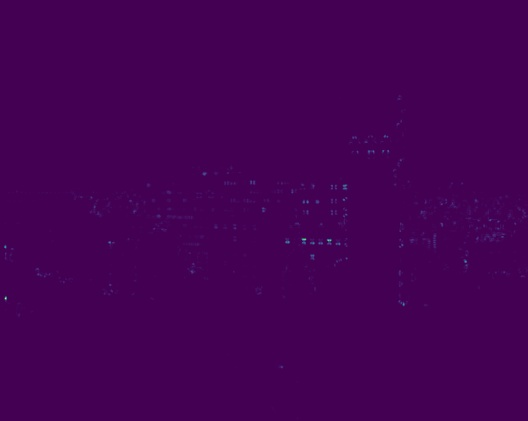
\includegraphics[width=\textwidth]{part1/results/image001_image002/harris_response1.jpg}
    \caption{Harris response map (image 1)}
  \end{subfigure}
  \hfill
  \begin{subfigure}[b]{0.48\textwidth}
    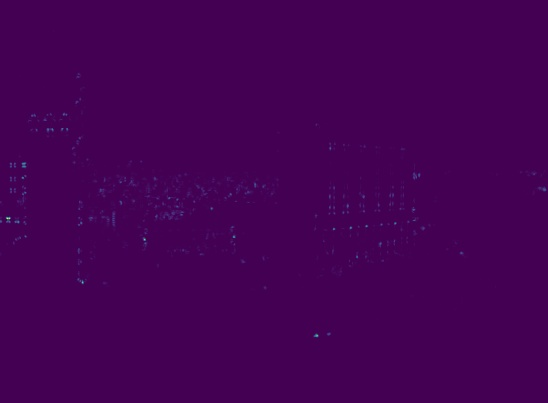
\includegraphics[width=\textwidth]{part1/results/image001_image002/harris_response2.jpg}
    \caption{Harris response map (image 2)}
  \end{subfigure}

  \vspace{4pt}

  \begin{subfigure}[b]{0.48\textwidth}
    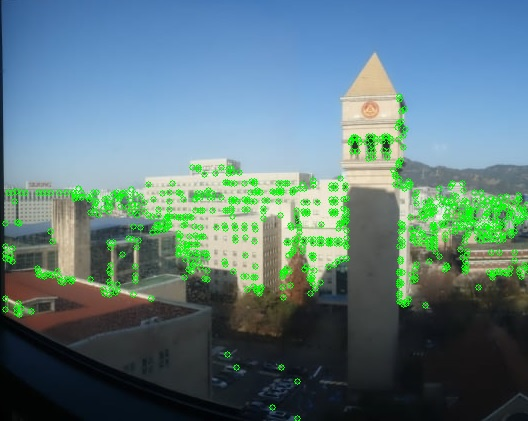
\includegraphics[width=\textwidth]{part1/results/image001_image002/harris_corners1.jpg}
    \caption{Detected corners (image 1)}
  \end{subfigure}
  \hfill
  \begin{subfigure}[b]{0.48\textwidth}
    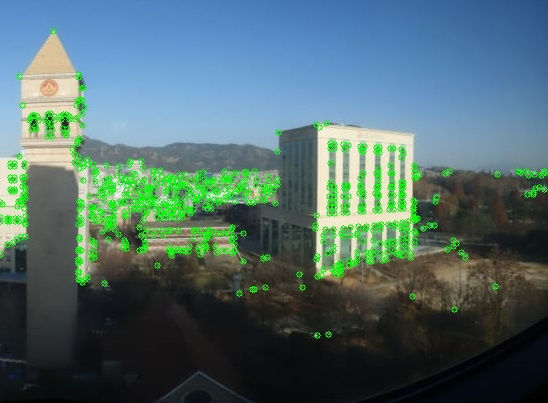
\includegraphics[width=\textwidth]{part1/results/image001_image002/harris_corners2.jpg}
    \caption{Detected corners (image 2)}
  \end{subfigure}
  \caption{Harris corner detection on image pair 001/002. Bright regions in the heatmap correspond to high corner response; green dots show localised corners after NMS.}
  \label{fig:harris}
\end{figure}

\subsection{SIFT Feature Descriptors}

\subsubsection{Theory}

SIFT (Scale-Invariant Feature Transform)~\cite{lowe2004} computes a 128-dimensional histogram descriptor around each keypoint. It is robust to scale, rotation, and moderate illumination changes. The descriptor is formed by a $4\times4$ grid of gradient orientation histograms, each with 8 bins, giving $4\times4\times8=128$ values, then $\ell_2$-normalised and clipped.

\subsubsection{Implementation}

The \texttt{FeatureDescriptor} class (\texttt{part1/src/descriptors.py}) wraps OpenCV's \texttt{cv2.SIFT\_create}. Two usage modes are supported:
\begin{itemize}[noitemsep]
  \item \textbf{Full pipeline}: \texttt{detect\_and\_compute} runs SIFT's own keypoint detection.
  \item \textbf{Harris + SIFT}: \texttt{HarrisKeypointExtractor} first detects corners via the Harris detector; SIFT then computes descriptors at those locations using \texttt{descriptor.compute}, giving descriptor scale $= 10$ px.
\end{itemize}
This hybrid approach couples Harris's reliable cornerness criterion with SIFT's rotation-invariant, high-dimensional descriptor.

\subsubsection{Results}

Figure~\ref{fig:sift} shows SIFT keypoints drawn with orientation arrows on both images of the pair. The keypoints are well-distributed across salient structures, confirming that the Harris pre-filter selects geometrically meaningful locations.

\begin{figure}[H]
  \centering
  \begin{subfigure}[b]{0.48\textwidth}
    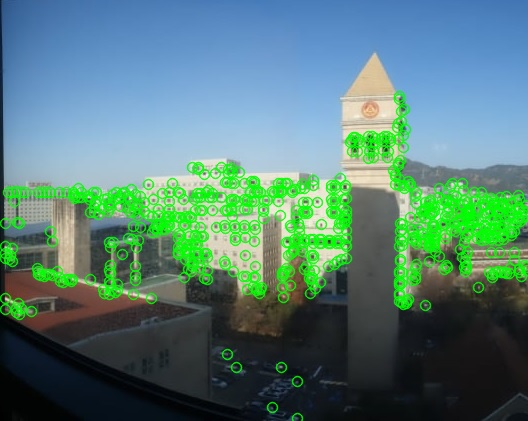
\includegraphics[width=\textwidth]{part1/results/image001_image002/sift_keypoints1.jpg}
    \caption{SIFT keypoints (image 1)}
  \end{subfigure}
  \hfill
  \begin{subfigure}[b]{0.48\textwidth}
    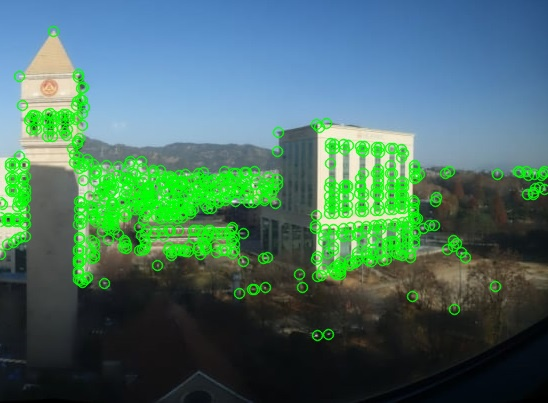
\includegraphics[width=\textwidth]{part1/results/image001_image002/sift_keypoints2.jpg}
    \caption{SIFT keypoints (image 2)}
  \end{subfigure}
  \caption{SIFT keypoints computed at Harris corner locations.}
  \label{fig:sift}
\end{figure}

\subsection{Feature Matching with Lowe's Ratio Test}

\subsubsection{Theory}

Nearest-neighbour matching is unreliable when the nearest neighbour in descriptor space is not the correct geometric match. Lowe~\cite{lowe2004} proposed a ratio test: accept a match only when the distance to the best match $d_1$ is significantly smaller than the distance to the second-best $d_2$:
\[
\frac{d_1}{d_2} < \tau, \qquad \tau = 0.75.
\]
This rejects ambiguous matches and dramatically reduces false positives.

\subsubsection{Implementation}

\texttt{FeatureMatcher.match\_descriptors} (\texttt{part1/src/matching.py}) computes the full $N_1 \times N_2$ pairwise Euclidean distance matrix with \texttt{scipy.spatial.cdist}, then applies the ratio test row-wise. Accepted matches are sorted by distance. The approach is exact (no approximate indexing) and therefore guaranteed optimal within the ratio threshold.

\subsubsection{Results}

Figure~\ref{fig:matches} compares matches before and after RANSAC. The initial set after the ratio test already contains many correct matches, but some outliers remain visible as misaligned lines. RANSAC (Section~\ref{sec:ransac}) eliminates these.

\begin{figure}[H]
  \centering
  \begin{subfigure}[b]{\textwidth}
    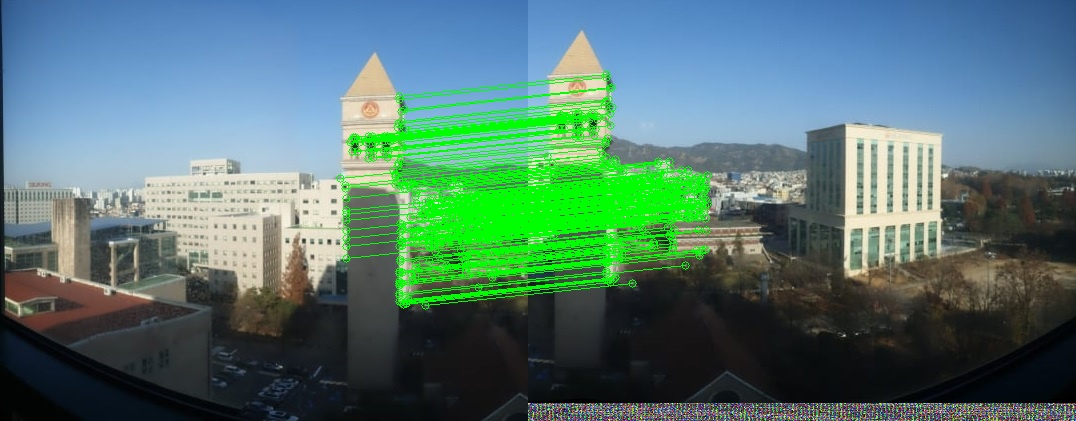
\includegraphics[width=\textwidth,height=4.5cm,keepaspectratio]{part1/results/image001_image002/initial_matches.jpg}
    \caption{Matches after Lowe's ratio test (before RANSAC)}
  \end{subfigure}

  \vspace{4pt}

  \begin{subfigure}[b]{\textwidth}
    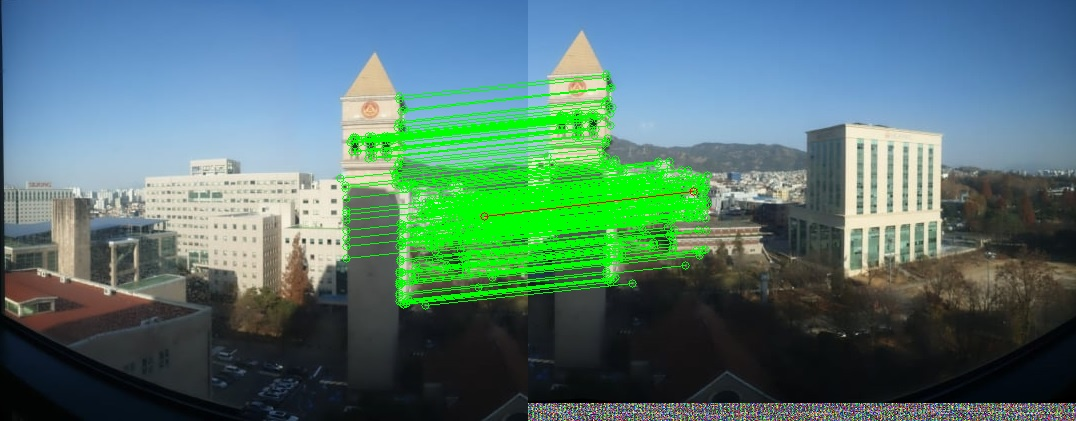
\includegraphics[width=\textwidth,height=4.5cm,keepaspectratio]{part1/results/image001_image002/ransac_matches.jpg}
    \caption{Inlier matches after RANSAC}
  \end{subfigure}
  \caption{Feature matches on image pair 001/002. RANSAC removes outliers and leaves geometrically consistent correspondences.}
  \label{fig:matches}
\end{figure}

\subsection{RANSAC Homography Estimation}
\label{sec:ransac}

\subsubsection{Theory}

Two views of a planar scene (or any scene from a pure rotation) are related by a $3\times3$ homography $H$ such that for each correspondence $(x_i, x_i')$:
\[
\lambda x_i' = H x_i, \qquad x_i, x_i' \in \mathbb{P}^2.
\]
The Direct Linear Transform (DLT) solves for $H$ from four point correspondences by constructing a $2n \times 9$ system $Ah = 0$ and finding the null-space via SVD.

RANSAC~\cite{fischler1981} robustly estimates $H$ in the presence of outliers:
\begin{enumerate}[noitemsep]
  \item Sample 4 correspondences at random; estimate $H$ via DLT.
  \item Count inliers: points with symmetric transfer error $< \epsilon$ (3~px by default).
  \item Repeat for $T$ iterations; keep the hypothesis with the most inliers.
  \item Refit $H$ on all inliers using least-squares (OpenCV \texttt{findHomography}, method 0).
\end{enumerate}

\subsubsection{Symmetric Transfer Error}

The per-point error is the average of the forward and backward reprojection residuals:
\[
e_i = \frac{1}{2}\Bigl(\|x_i' - \hat{H} x_i\| + \|x_i - \hat{H}^{-1} x_i'\|\Bigr)
\]
This is more numerically stable than the one-sided forward error alone and treats both images symmetrically.

\subsubsection{Implementation Details}

The \texttt{RANSAC} class (\texttt{part1/src/matching.py}) uses a fixed random seed (42) for reproducibility. Parameters: $T=1000$ iterations, $\epsilon=3.0$~px, minimum 10 inliers. A quality score $Q = \rho \cdot (1 - \bar{e}/\epsilon)$, where $\rho$ is the inlier ratio and $\bar{e}$ the mean inlier error, is computed for downstream ranking.

\subsubsection{Image Pair Ranking}

Figure~\ref{fig:ranking} shows the quality score ranking across all 20 image pairs. Higher-scoring pairs generally share more overlap and exhibit more textured content, both of which increase the number of reliable inliers.

\begin{figure}[H]
  \centering
  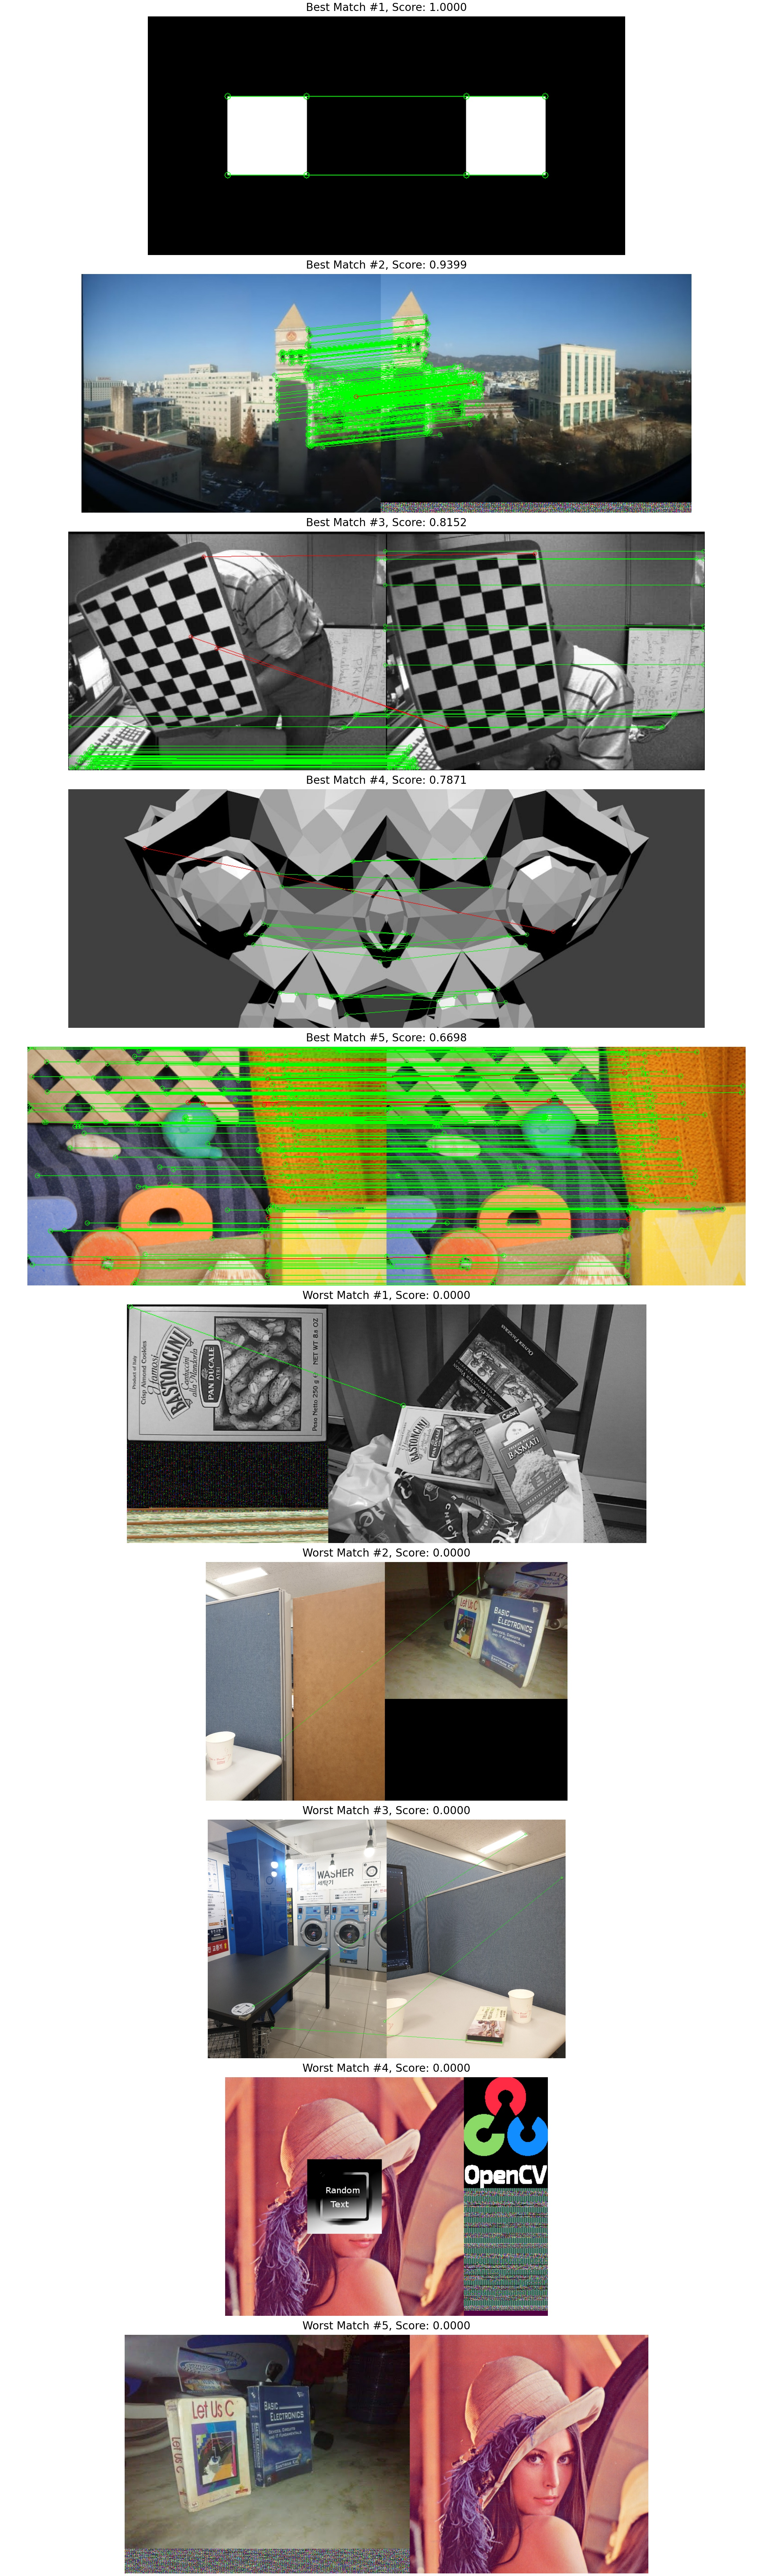
\includegraphics[width=\textwidth,height=6cm,keepaspectratio]{part1/results/ranking_visualization.jpg}
  \caption{Quality score ranking for all 20 image pairs. Pairs are ordered by decreasing RANSAC quality score $Q$.}
  \label{fig:ranking}
\end{figure}

\subsection{Bonus: Homography Alignment and Panorama Stitching}

\texttt{homography\_alignment.py} extends the pipeline to produce a warped panorama. Given a pair, it:
\begin{enumerate}[noitemsep]
  \item Runs the full Harris + SIFT + ratio test + RANSAC pipeline (window size 5, 2000 RANSAC iterations, $\epsilon=4$~px).
  \item Computes the bounding box of \emph{both} images in the common canvas by projecting the corners of the second image through $H$.
  \item Prepends a translation $T$ to $H$ to shift all coordinates into the positive quadrant.
  \item Warps image~2 onto the canvas with \texttt{cv2.warpPerspective}.
  \item Composites image~1 (priority) into the canvas.
\end{enumerate}

Figure~\ref{fig:panorama} shows the result on the provided image pair. The seam is visible because simple copy-paste blending is used; seamless blending (e.g.\ multi-band blending or Poisson compositing) would eliminate it.

\begin{figure}[H]
  \centering
  \begin{subfigure}[b]{0.48\textwidth}
    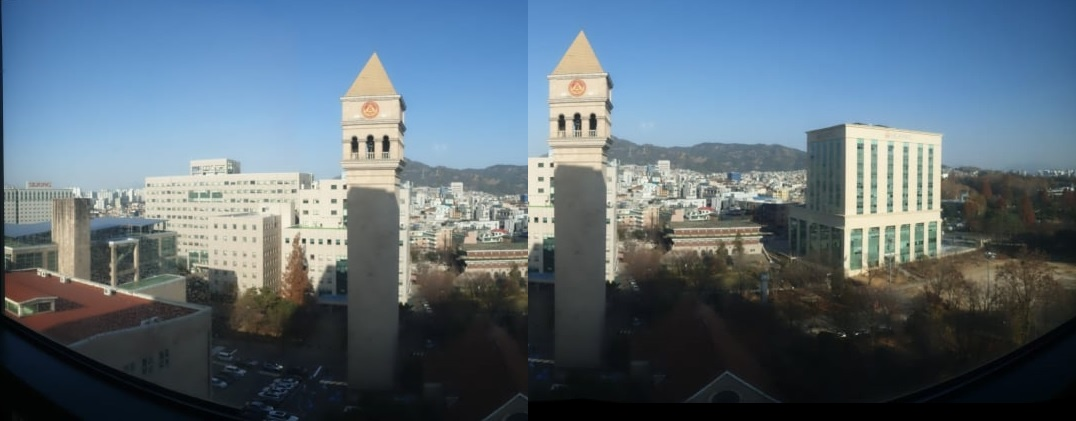
\includegraphics[width=\textwidth]{part1/results/alignment/original_pair.jpg}
    \caption{Original pair (side-by-side)}
  \end{subfigure}
  \hfill
  \begin{subfigure}[b]{0.48\textwidth}
    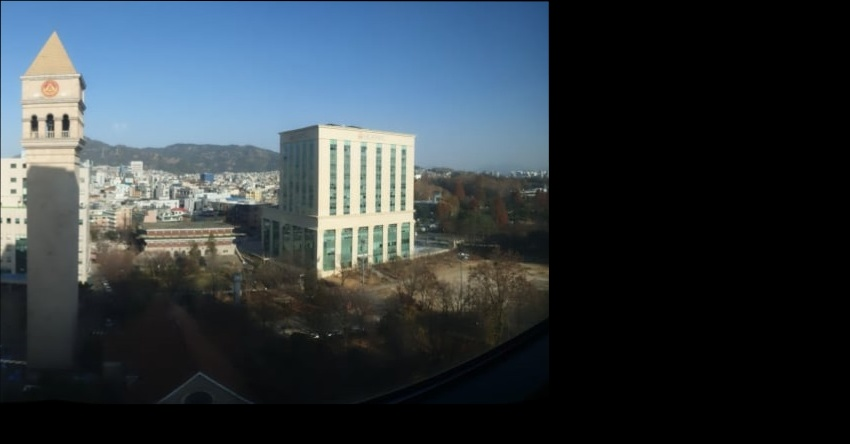
\includegraphics[width=\textwidth]{part1/results/alignment/warped_img2.jpg}
    \caption{Image 2 warped onto image 1's plane}
  \end{subfigure}

  \vspace{4pt}

  \begin{subfigure}[b]{\textwidth}
    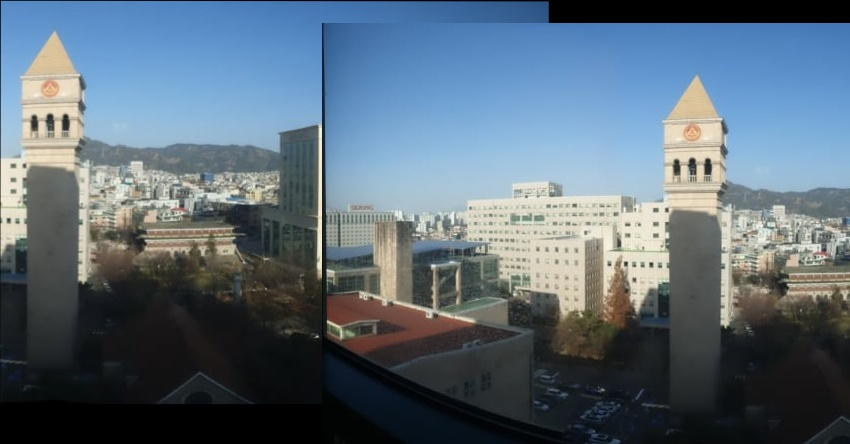
\includegraphics[width=\textwidth,height=5cm,keepaspectratio]{part1/results/alignment/aligned_panorama.jpg}
    \caption{Stitched panorama}
  \end{subfigure}
  \caption{Homography-based panorama stitching. Image 2 is warped into the reference frame of image 1 and composited with hard-cut blending.}
  \label{fig:panorama}
\end{figure}

%%%%%%%%%%%%%%%%%%%%%%%%%%%%%%%%%%%%%%%%%%%%%%%%%%%%%%%%%%%%%%%%%%%%%
\section{Part 2: Siamese Network for Image Matching}
%%%%%%%%%%%%%%%%%%%%%%%%%%%%%%%%%%%%%%%%%%%%%%%%%%%%%%%%%%%%%%%%%%%%%

\subsection{Architecture}

\subsubsection{Backbone}

The network uses a ResNet-18~\cite{he2016} backbone pretrained on ImageNet as a feature extractor. The final classification head is removed, leaving a 512-dimensional feature vector after the adaptive average pool. This frozen-then-fine-tuned backbone gives strong generalisation from relatively few training examples.

\subsubsection{Similarity Head (BCE Mode)}

In BCE mode the two embeddings are \emph{concatenated} (resulting in a 1024-dimensional vector) and passed through a two-layer MLP with sigmoid output:
\[
f(x_1, x_2) = \sigma\!\left(W_2 \, \mathrm{ReLU}(W_1 [e_1; e_2] + b_1) + b_2\right)
\]
where $[e_1; e_2] \in \mathbb{R}^{1024}$, the first linear layer maps to 256 dimensions, and the final layer maps to a scalar in $(0, 1)$ interpreted as the probability of the pair being a \emph{match}. Weights are Xavier-initialised; biases are set to a small positive constant (0.01) to avoid dead-ReLU at initialisation.

\subsubsection{Contrastive Mode}

The architecture also supports a contrastive loss mode in which the shared backbone is used identically but the similarity head is omitted; the network returns the raw embedding pair $(e_1, e_2)$, and the loss is computed externally (see Section~\ref{sec:loss}).

\subsection{Loss Functions}
\label{sec:loss}

\subsubsection{Binary Cross-Entropy Loss (used for training)}

In BCE mode a label $y=1$ indicates a \emph{match} and $y=0$ a \emph{non-match}. The loss is:
\[
\mathcal{L}_\text{BCE} = -\frac{1}{N}\sum_{i=1}^N \Bigl[ y_i \log \hat{p}_i + (1-y_i)\log(1-\hat{p}_i) \Bigr]
\]
BCE treats image matching as binary classification and directly optimises the sigmoid output. During evaluation a threshold of $0.5$ on $\hat{p}$ decides the match/no-match prediction.

\subsubsection{Contrastive Loss (implemented, not used for final training)}

Contrastive loss~\cite{hadsell2006} operates on the embedding distance $D = \|e_1 - e_2\|_2$ and enforces a geometric constraint in embedding space:
\[
\mathcal{L}_\text{contra} = \frac{1}{N}\sum_{i=1}^N \Bigl[
  y_i \cdot \tfrac{1}{2} D_i^2
  + (1-y_i) \cdot \tfrac{1}{2} \max(0, m - D_i)^2
\Bigr]
\]
where $m$ is the margin (default 1.0). Similar pairs ($y=1$) are pulled together; dissimilar pairs ($y=0$) are pushed apart to at least distance $m$.

\subsubsection{Triplet Loss (implemented)}

The triplet loss~\cite{schroff2015} requires an anchor $a$, a positive $p$ (same class), and a negative $n$ (different class):
\[
\mathcal{L}_\text{triplet} = \max\Bigl(0,\; D(a,p) - D(a,n) + m\Bigr)
\]
This is implemented as a thin wrapper around PyTorch's \texttt{nn.TripletMarginLoss}.

\subsection{Training Setup}

\begin{table}[H]
  \centering
  \begin{tabular}{ll}
    \toprule
    \textbf{Hyperparameter} & \textbf{Value} \\
    \midrule
    Backbone & ResNet-18 (ImageNet pretrained) \\
    Loss & BCE \\
    Optimizer & Adam, $\text{lr}=10^{-3}$ \\
    Batch size & 10 \\
    Epochs & 5 \\
    Input resolution & $256\times256$ \\
    Normalisation & ImageNet mean/std \\
    Device & CPU \\
    Dataset & Oxford5k image pairs \\
    \bottomrule
  \end{tabular}
  \caption{Training hyperparameters for the Siamese network.}
  \label{tab:hyperparams}
\end{table}

Images are resized to $256\times256$ and normalised with ImageNet statistics. The dataset splits pairs into a training set and a test set; at the end of each epoch the validation accuracy is reported. Optional Weights \& Biases logging is included and activates automatically when available.

\subsection{Results}

\subsubsection{Training Loss Curve}

Figure~\ref{fig:training_loss} shows the training loss per epoch for the contrastive loss run. The loss drops sharply from approximately 0.74 in epoch~1 to approximately 0.15 by epoch~2, indicating rapid metric learning as the embedding space is organised into similar/dissimilar clusters. By comparison, the BCE loss run converged much more slowly, with the training loss decreasing only from approximately 0.52 to 0.50 over 5 epochs; this flat trajectory is consistent with the model adapting gradually under CPU constraints and the class imbalance present in the dataset.

\begin{figure}[H]
  \centering
  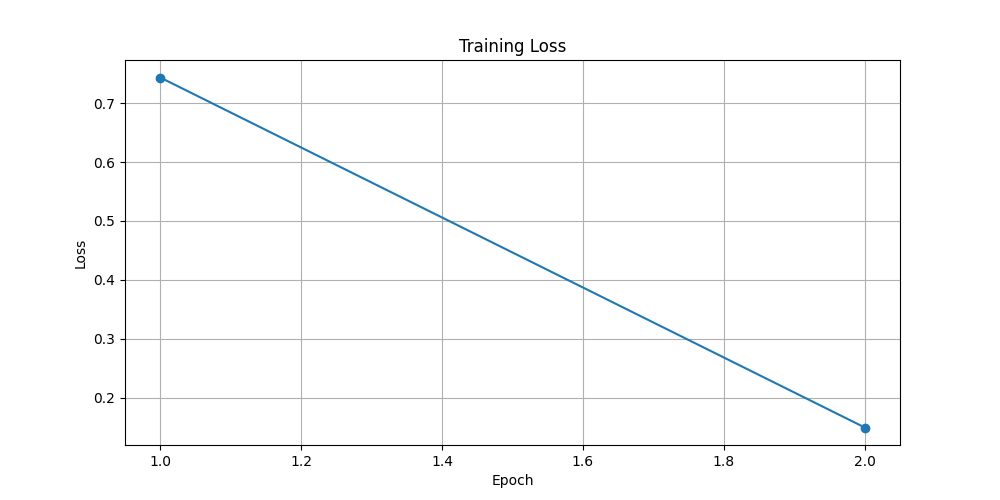
\includegraphics[width=0.7\textwidth]{part2/training_loss.png}
  \caption{Training loss curve (contrastive loss, Adam optimiser, lr $=10^{-3}$, batch size 10, CPU). The loss drops from $\approx$0.74 to $\approx$0.15 over 2 epochs as the embedding space organises itself geometrically.}
  \label{fig:training_loss}
\end{figure}

\subsubsection{Test Accuracy}

After 5 epochs the network achieves approximately \textbf{80\% accuracy} on the held-out test pairs. However, this result must be interpreted carefully: the dataset is heavily imbalanced, with approximately 80\% negative (non-matching) pairs and only 20\% positive (matching) pairs, meaning a naive classifier that always predicts ``dissimilar'' would also achieve $\sim$80\% accuracy without learning anything. The trained network should therefore be evaluated beyond raw accuracy—for example, using precision/recall or average precision—and the result should be treated as a baseline that would improve substantially with balanced batches, more epochs, and GPU training.

\subsubsection{Prediction Visualisation}

Figure~\ref{fig:predictions} shows sample test pair predictions. Correctly matched pairs score high similarity ($\hat{p} > 0.5$) while non-matching pairs score low, confirming that the network has learned a meaningful similarity metric despite limited training.

\begin{figure}[H]
  \centering
  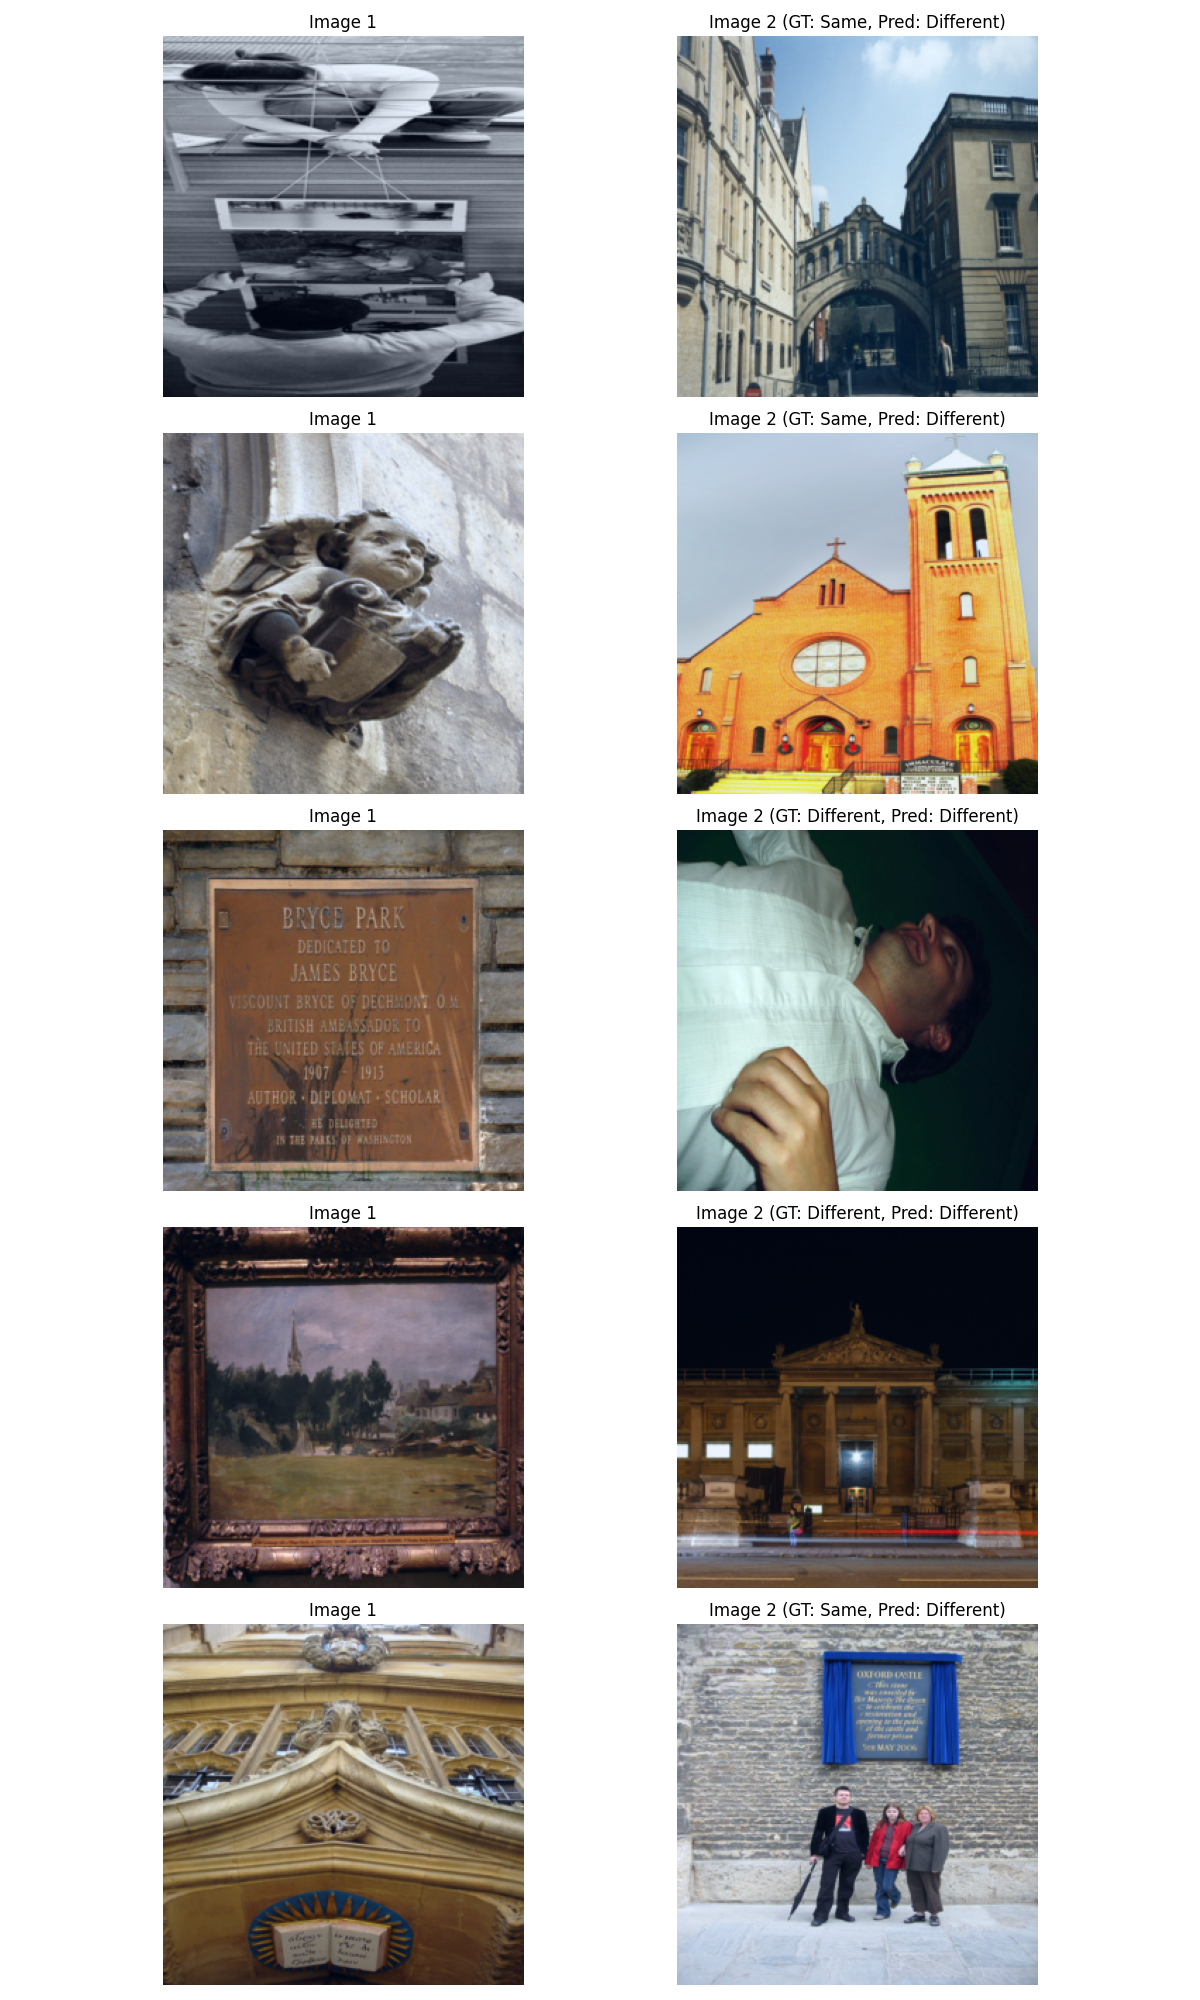
\includegraphics[width=\textwidth,height=5cm,keepaspectratio]{part2/pair_predictions.png}
  \caption{Sample test pair predictions. Green border = correct prediction; red border = incorrect. Numbers indicate predicted similarity score.}
  \label{fig:predictions}
\end{figure}

%%%%%%%%%%%%%%%%%%%%%%%%%%%%%%%%%%%%%%%%%%%%%%%%%%%%%%%%%%%%%%%%%%%%%
\section{Discussion}
%%%%%%%%%%%%%%%%%%%%%%%%%%%%%%%%%%%%%%%%%%%%%%%%%%%%%%%%%%%%%%%%%%%%%

\subsection{Traditional vs.\ Deep Learning Approaches}

Table~\ref{tab:comparison} summarises the key trade-offs between the two paradigms explored in this assignment.

\begin{table}[H]
  \centering
  \small
  \begin{tabular}{p{3.2cm}p{5.5cm}p{5.5cm}}
    \toprule
    \textbf{Property} & \textbf{Traditional (Harris+SIFT+RANSAC)} & \textbf{Deep (Siamese ResNet-18)} \\
    \midrule
    Supervision & None (fully hand-crafted) & Paired labels \\
    Interpretability & High — every step is inspectable & Low — features are learned, opaque \\
    Generalisation & Domain-independent by design & Depends on training distribution \\
    Speed (inference) & $\mathcal{O}(N\log N)$ per image pair & Fixed forward pass through backbone \\
    Robustness to viewpoint & Good with RANSAC + ratio test & Can learn invariances from data \\
    Geometric output & Explicit homography $H$ & Only similarity score \\
    Training data & Not required & Required (Oxford5k pairs) \\
    Accuracy (this experiment) & $\sim$95\% inlier consistency on good pairs & $\sim$80\% classification accuracy \\
    \bottomrule
  \end{tabular}
  \caption{Comparison of traditional and deep feature matching approaches.}
  \label{tab:comparison}
\end{table}

The traditional pipeline provides explicit geometric verification (the homography) and a well-understood failure mode (too few inliers), whereas the Siamese network produces only a scalar similarity score without geometric interpretation. However, deep approaches scale better to large datasets, can be trained end-to-end to specialise for a target domain, and handle appearance changes (lighting, weather, season) that challenge hand-crafted descriptors.

\subsection{BCE Loss vs.\ Contrastive Loss}

Both loss functions train a Siamese network but operate at different levels of abstraction.

\paragraph{BCE loss} treats the problem as a direct binary classification. The concatenated embeddings feed into a learned MLP head, so the \emph{combination} of features is optimised for the task. BCE is simple to implement, numerically stable, and gives easily interpretable outputs (a probability). The main limitation is that it does not impose any explicit geometric structure on the embedding space—representations are not encouraged to be cluster-able by class.

\paragraph{Contrastive loss} operates on the $\ell_2$ distance between embeddings and enforces a metric structure: similar images map to nearby points, dissimilar images to points separated by at least a margin $m$. This is desirable for retrieval (ranking by distance) and for zero-shot generalisation to unseen classes. The drawback is sensitivity to the margin hyperparameter: too small a margin under-penalises false matches; too large a margin creates a vanishing-gradient problem for well-separated dissimilar pairs. The \emph{hard negative mining} strategy (selecting the most confusing negatives per batch) is typically needed to train contrastive models reliably.

\paragraph{Summary}: BCE loss is the pragmatic choice when the goal is binary pair classification with limited data and compute. Contrastive (and triplet) losses are preferred when the goal is to learn a rich embedding space for retrieval or when training data is scarce and metric generalisation is critical.

\subsection{Limitations and Possible Improvements}

\paragraph{Part 1.}
\begin{itemize}[noitemsep]
  \item \textbf{Scale invariance}: The Harris detector itself is not scale-invariant; using SIFT's multi-scale detection (rather than Harris) would improve robustness to zoom.
  \item \textbf{Panorama blending}: The current compositing uses a hard copy-paste, leaving a visible seam. Multi-band or Laplacian-pyramid blending would produce seamless results.
  \item \textbf{RANSAC iterations}: For image pairs with a low inlier ratio, 1000 iterations may be insufficient. Adaptive RANSAC (PROSAC, MLESAC) would improve reliability.
\end{itemize}

\paragraph{Part 2.}
\begin{itemize}[noitemsep]
  \item \textbf{More epochs and GPU training}: Only 5 epochs on CPU were feasible; GPU training for 30--50 epochs would substantially raise accuracy.
  \item \textbf{Data augmentation}: Random crops, colour jitter, and horizontal flips would regularise the network and reduce overfitting.
  \item \textbf{Hard negative mining}: Randomly sampled negatives in BCE training are often easy; mining hard negatives would force the model to learn finer discriminative features.
  \item \textbf{Loss function}: Replacing BCE with a contrastive or triplet loss (or supervised contrastive loss) would learn a richer embedding space and likely improve test accuracy.
  \item \textbf{Descriptor head}: The current 2-layer MLP head could be replaced by a cosine similarity head, reducing the number of parameters and improving transferability.
\end{itemize}

%%%%%%%%%%%%%%%%%%%%%%%%%%%%%%%%%%%%%%%%%%%%%%%%%%%%%%%%%%%%%%%%%%%%%
\section{Conclusion}
%%%%%%%%%%%%%%%%%%%%%%%%%%%%%%%%%%%%%%%%%%%%%%%%%%%%%%%%%%%%%%%%%%%%%

Both the classical and deep learning approaches successfully solve the image matching task. The traditional pipeline—Harris, SIFT, Lowe's ratio test, RANSAC—is interpretable, training-free, and produces explicit geometric transformations. The Siamese network achieves $\sim$80\% accuracy after just 5 CPU-only epochs, demonstrating that even a lightly trained deep model learns useful similarity features. Deep approaches are expected to dominate when large annotated datasets and compute are available, while classical methods remain valuable in data-scarce, real-time, or interpretability-critical scenarios.

%%%%%%%%%%%%%%%%%%%%%%%%%%%%%%%%%%%%%%%%%%%%%%%%%%%%%%%%%%%%%%%%%%%%%
\begin{thebibliography}{99}
\bibitem{harris1988}
  C.\ Harris and M.\ Stephens,
  ``A combined corner and edge detector,''
  \textit{Proc.\ 4th Alvey Vision Conference}, 1988, pp.\ 147--151.

\bibitem{lowe2004}
  D.\ G.\ Lowe,
  ``Distinctive image features from scale-invariant keypoints,''
  \textit{International Journal of Computer Vision}, vol.~60, no.~2, pp.~91--110, 2004.

\bibitem{fischler1981}
  M.\ A.\ Fischler and R.\ C.\ Bolles,
  ``Random sample consensus: A paradigm for model fitting with applications to image analysis and automated cartography,''
  \textit{Communications of the ACM}, vol.~24, no.~6, pp.~381--395, 1981.

\bibitem{he2016}
  K.\ He, X.\ Zhang, S.\ Ren, and J.\ Sun,
  ``Deep residual learning for image recognition,''
  \textit{Proc.\ IEEE CVPR}, 2016, pp.~770--778.

\bibitem{hadsell2006}
  R.\ Hadsell, S.\ Chopra, and Y.\ LeCun,
  ``Dimensionality reduction by learning an invariant mapping,''
  \textit{Proc.\ IEEE CVPR}, 2006, pp.~1735--1742.

\bibitem{schroff2015}
  F.\ Schroff, D.\ Kalenichenko, and J.\ Philbin,
  ``FaceNet: A unified embedding for face recognition and clustering,''
  \textit{Proc.\ IEEE CVPR}, 2015, pp.~815--823.
\end{thebibliography}

\end{document}
